\documentclass[xelatex,ja=standard,jafont=noto]{bxjsarticle}
\usepackage[utf8]{inputenc}

\date{11.4 2020}

\usepackage{natbib}
\usepackage{graphicx}
\usepackage{tikz}
\usepackage{circuitikz}
\usepackage{tabularx}
\usepackage{diagbox}
\usepackage{amsmath,amssymb}
\numberwithin{figure}{section}
\usepackage{pdfpages}

\usepackage{hyperref}


\begin{document}
\renewcommand{\figurename}{Fig.}
\renewcommand{\tablename}{Table }



	\begin{titlepage}
			\begin{center}
				
				{\Large 令和2年}
				
				\vspace{10truept}
				
				{\Large 機械工学実験2}
				
				\vspace*{140truept}
				
				{\Huge モータシステムの制御系設計} 
				
				\vspace{160truept}
				
				{\Large 指導教員}
				
				\vspace{10truept}
				
				{\Large  Ito Kazuhisa }
				
				\vspace{70truept}
				{\Large 芝浦工業大学}
				
				\vspace{10truept}
				
				{\Large 機械制御システム}
				
				\vspace{30truept}
				
				{\Large bq18026 関宇}      
				
			\end{center}
		\end{titlepage}
%\includepdf[pages={1}]{sd.pdf}


\tableofcontents

\newpage



\section{図 1 に示すブロック線図において}

\begin{figure}[h!]
    \centering
    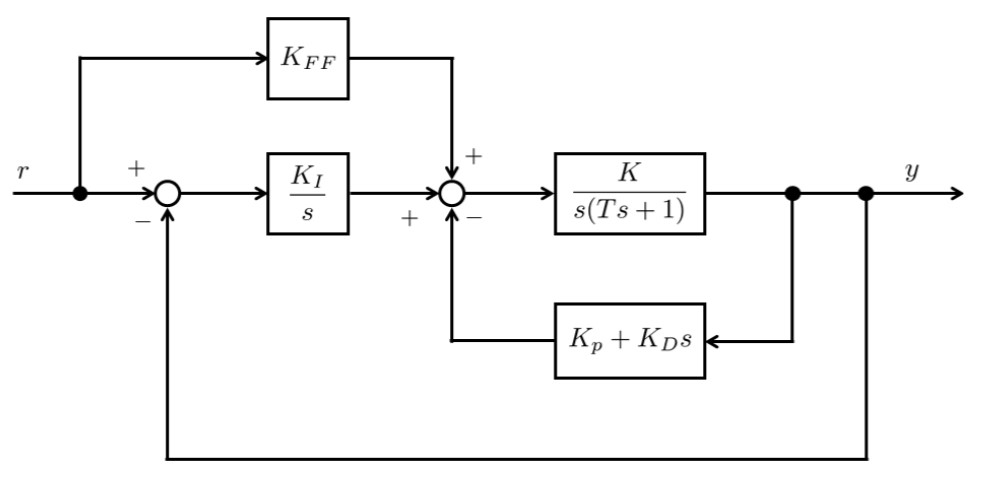
\includegraphics[scale=0.6]{01.jpg}
    \caption{I-PD+FF 制御系 }
\end{figure}

\subsection{r から y までの伝達関数を求めよ.}
まずこのブロック線図内のフィードバック系$ G_{1}(s) $の伝達関数を求める.

\begin{equation}
    G_{1}(s)=\frac{\frac{k}{s(Ts+1)}}{1+\frac{k(k_{p}+K_{D}s)}{s(Ts+1)}}
\end{equation}

\begin{equation}
    G_{1}(s)=\frac{k}{s^{2}T+(k_{D}+1)s+kk_{p}}
\end{equation}

よって、図1はこのように表すことができる.

\begin{figure}[h!]
    \centering
    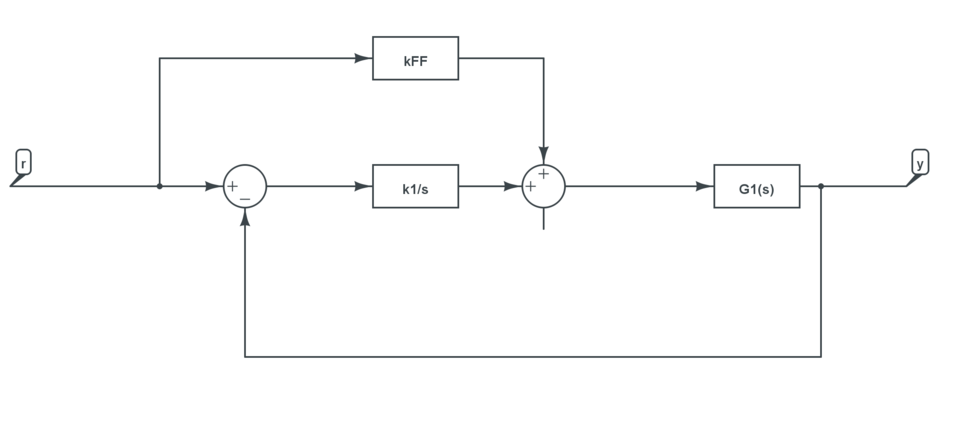
\includegraphics[scale=0.4]{012.png}
    \caption{I-PD+FF 制御系 }
\end{figure}

さらに,ブロック線図の等価変化から,次のように表すことができる.

\newpage

\begin{figure}[h!]
    \centering
    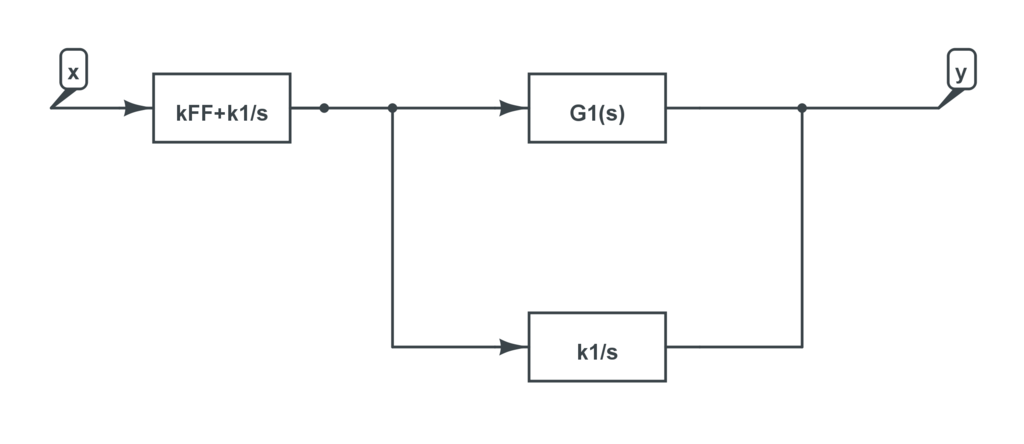
\includegraphics[scale=0.4]{013.png}
    \caption{I-PD+FF 制御系 }
\end{figure}

よって、伝達関数$ G(s) $は

\begin{equation}
    G(s)=(k_{FF}+\frac{K_{I}}{s})\cdot\frac{\frac{k}{s^{2}T+(kk_{D}+1)s+kk_{p}}}{1+\frac{kk_{I}}{s(s^{2}T+(kk_{D}+1)s+kk_{p})}}
\end{equation}\\

\begin{equation}
    G(s)=\frac{k_{I}k+k_{FF}ks}{s^{3}T+s^{2}(kk_{D}+1)+kk_{P}s+kk_{I}}
\end{equation}

\subsection{伝達関数の極}

(i) で求めた伝達関数の極を$ p_{1}=-\alpha,p_{2}=-\zeta\omega_{n}+j\omega_{n}\sqrt{1-\zeta^{2}},p_{3}=-\zeta\omega_{n}-j\omega_{n}\sqrt{1-\zeta^{2}}     $としたとき,係数比較により KP,KI,KD を$\zeta,\omega_{n},\alpha $で表せ.\\


関数の極を特性多項式に代入して、

\begin{equation}
    (s+\alpha)(s^{2}+2\zeta\omega_{n}s+\omega_{n}^{2})
\end{equation}

その特性多項式を展開し

\begin{equation}
    =s^{3}+2s^{2}\zeta\omega_{n}+s\omega_{n}^{2}+s^{2}\alpha+2\zeta\omega_{n}s\alpha+\alpha\omega_{n}^{2}
\end{equation}

\begin{equation}
    =s^{3}+s^{2}(2\zeta\omega_{n}+\alpha)+s(\omega_{n}^{2}+2\zeta\omega_{n}\alpha)+\alpha\omega_{n}^{2}
\end{equation}


それを4で求めた伝達関数の特性多項式と比べて

\begin{equation}
    T=1;K_{I}=\frac{\alpha\omega_{n}^{2}}{K};K_{D}=\frac{2\zeta\omega_{n}+\alpha-1}{K};K_{P}=\frac{\omega_{n}^{2}+2\zeta\omega_{n}\alpha}{K}
\end{equation}



\subsection{(ii) で与えた極と結果を用いて,$K_{FF}=K_{I}/\alpha$ としたときの伝達関数を求めよ.}


\newpage

(7)の結論を式4に代入して

\begin{equation}
    G(s)=\frac{\omega_{n}^{2}(s+\alpha)}{s^{3}+s^{2}(2\zeta\omega_{n}+\alpha)+s(\omega_{n}^{2}+2\zeta\omega_{n}\alpha)+\alpha\omega_{n}^{2}}
\end{equation}


\section{二次遅れ系の $ \zeta,\omega_{n}$ と最大オーバーシュート量および 5パーセント整定時間との関係を示せ.}

\subsection{最大オーバーシュート時間}\\

最大オーバーシュートの箇所ではステップ応答の時間微分は0となる.よって、ステップ応答を表す式の時間微分を求めて、その式の値が0となる時間を求めれば、最大オーバーシュート時間を算出することができる.\\

 

ステップ応答の時間微分を表す式は、

\begin{equation}
    \Dot{g}(t)=\frac{1}{\sqrt{1-\zeta^{2}}}e^{-\zeta\omega_{n}t}sin(\omega_{n}\sqrt{1-\zeta^{2}}t)
\end{equation}

    この式の値を0となるため、
    
    \begin{equation}
        \omega_{n}\sqrt{1-\zeta^{2}}t=n\pi
    \end{equation}
    
    これより、最大オーバーシュート時間Tは、
    
    \begin{equation}
        T=\frac{\pi}{\omega_{n}\sqrt{1-\zeta^{2}}}
    \end{equation}

\subsection{最大オーバーシュート量}

最大オーバーシュート量OSは、時間領域tでのステップ応答の最大値gmaxと応答の最終値gfinalの関係を

\begin{equation}
    OS=100\cdot\frac{gmax-gfinal}{gfinal}
\end{equation}

特に、

\begin{equation}
    gmax=1+e^{-\frac{\zeta\pi}{\sqrt{1-\zeta^{2}}}}
\end{equation}

ステップ応答の最終値gfinalは1なので、これより最大オーバーシュート量OSは、

\begin{equation}
    OS=100e^{-\frac{\zeta\pi}{\sqrt{1-\zeta^{2}}}}
\end{equation}

\newpage


\section{機械制御におけるワインドアップ現象について図を用いて説明し,その対策について述べよ.}

\subsection{ワインドアップとは}

\begin{figure}[h!]
    \centering
    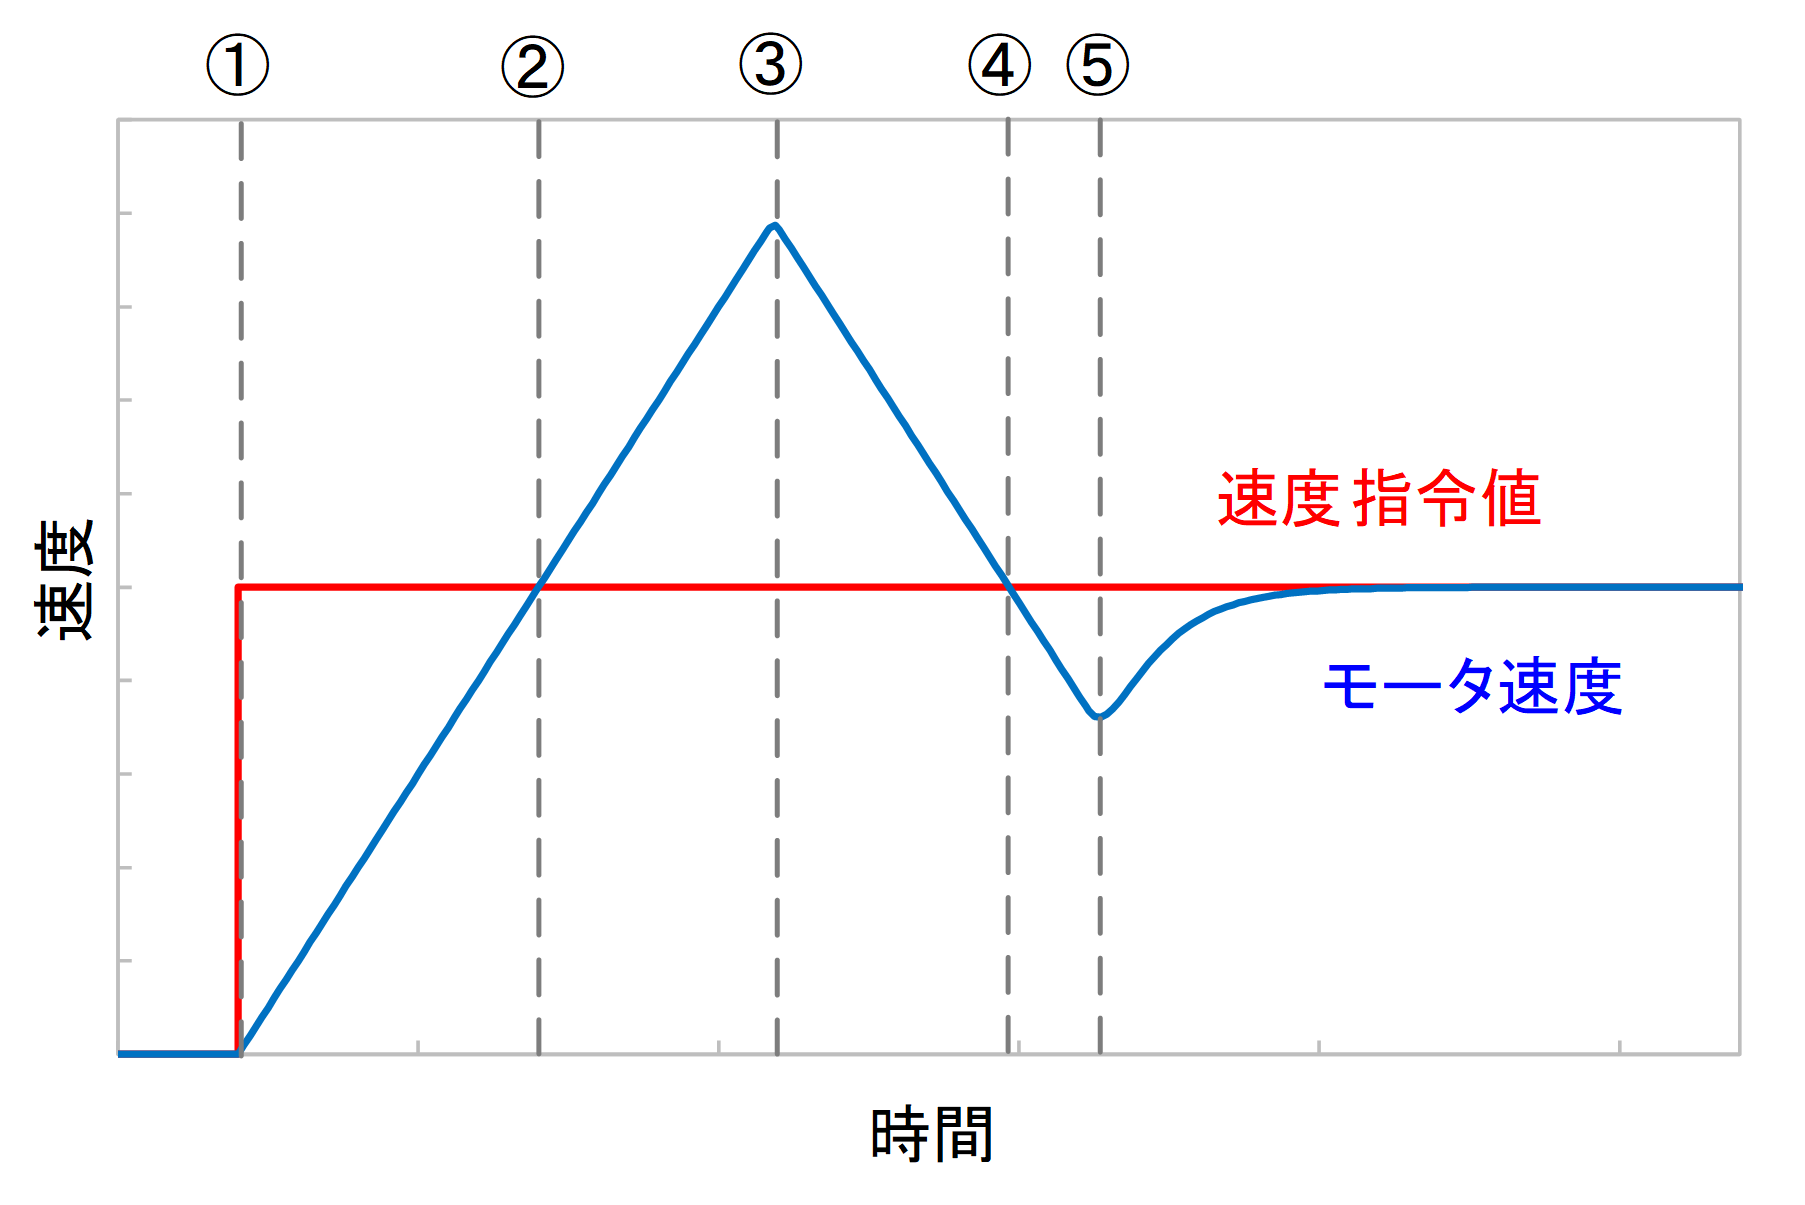
\includegraphics[scale=0.8]{014.png}
    \caption{リミッタを含むシステムにおける速度ステップ応答 }
\end{figure}


図の1でステップ速度指令が入力されると、PI制御器はステップ状のモータ速度応答を実現するためにインパルス状のトルクを出力しようとする.しかし、リミッタによって出力トルクが制限されるため、実際には図の1から2の区間のようなランプ状の速度応答となる.この速度の傾き(加速度)は出力可能なトルクによって決める.モータ速度が目標速度までランプ状に増加している間、積分器は偏差を積分し続ける.モータ速度が目標速度に達した後は、偏差の正負が逆転するため積分器に蓄積された値は減少していきますが、加速時に蓄積された過大な値(積分操作量)が減少するまでの間、速度にオーバーシュートが発生します(2から4の区間).このことをワインドアップ(wind-up)現象と言う.ワインドアップ現象は、制御器出力がリミッタによって制限されて出力されることで、制御器の内部状態変数が実際の制御対象の状態量に対して不適切な値となることが主な原因となる.

\subsection{対策}

\begin{figure}[h!]
    \centering
    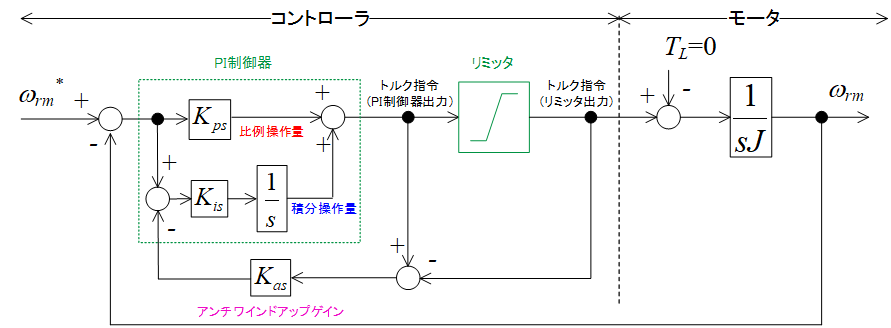
\includegraphics[scale=0.6]{015.png}
    \caption{リミット偏差フィードバック補償法のブロック図}
\end{figure}

ワインドアップ現象を回避する方法の一つであるリミット偏差フィードバック補償法のブロック図を示す.図のシステムではリミッタによって出力が制限されているのにも関わらず、制御器は過大な出力をし続ける.これは、制御器には「リミッタによって出力が制限されている」という情報が反映されていないため起こる現象だと考えることができる.リミッタ前後の差分をとることで実際の制御対象の状態量と制御器の内部状態変数の差を求めることができるため、この情報を制御器の積分偏差にフィードバックすれば、積分器に過大な値を蓄積を防ぐことができる.

\section{実験データ取得の際のサンプリング時間を決める手順について説明せよ.}

データ取得の際のサンプリングの周波数は必ず制御対象の2倍以上、つまり必ず一周期の半分以下である.理由は図のように表している.

\begin{figure}[h!]
    \centering
    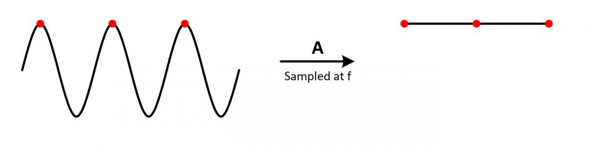
\includegraphics[scale=0.5]{016.png}
    \caption{fs=fn}
\end{figure}

\begin{figure}[h!]
    \centering
    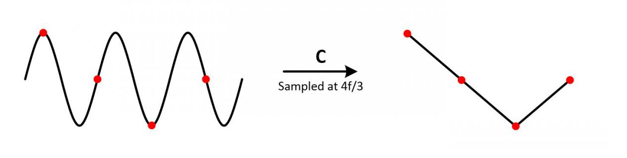
\includegraphics[scale=0.5]{017.png}
    \caption{fs=(4/3)fn}
\end{figure}

\begin{figure}[h!]
    \centering
    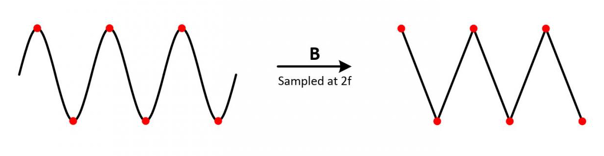
\includegraphics[scale=0.5]{018.png}
    \caption{fS=2fN}
\end{figure}



\newpage

\begin{thebibliography}{9}
\bibitem{latexcompanion} 
日本機械学会,制御工学,JSMEテキストシリ,2010/8/31,p.19.20. 

\bibitem{latexcompanion} 
黒川一夫,ロボット用回路駆動設計,工学研究社,2007/10/22,p.4. 


\bibitem{einstein} 
Embedded Technology Lab,ワインドアップ現象とその対策,
\url{https://nagaoka-md.co.jp/2020/07/16/pmsm-foc-no9/},参考日:2020/11/4



\end{thebibliography}





\end{document}